
%\documentclass{beamer} %voce pode usar este modelo tambem
\documentclass[handout,t]{beamer}
\usepackage{graphicx,url}
\usepackage[spanish]{babel}   
\usepackage[utf8]{inputenc}
\usepackage[backend=biber]{biblatex}
\usepackage{csquotes}
\usepackage{ragged2e}
\usepackage{comment}

\AtBeginBibliography{\tiny}
\bibliography{Referencias}
\useoutertheme{infolines}
\batchmode
\usepackage{amsmath,amssymb,enumerate,epsfig,bbm,calc,color,ifthen,capt-of}
\usetheme{Frankfurt}
\usecolortheme{whale}

\AtBeginSection[]
{
  \begin{frame}<beamer>
    \frametitle{Outline}
    \tableofcontents[currentsection]
  \end{frame}
}
\beamerdefaultoverlayspecification{<+->}
% -----------------------------------------------------------------------------
\begin{document}
% -----------------------------------------------------------------------------
%\institute[Posgrado en Ingeniería Eléctrica - UNAM]
%\section{}
\begin{frame}{}
\phantom{sd}\\
\phantom{sd}\\
\centering\textbf{{\Large Percepción Artificial y Planeación de Acciones a partir de la cámara RGBD de un Robot Móvil}}
\\

\phantom{sd}\\
\emph{Presenta:\\ Ing. Mitzi Anaid Ramírez Estrada\\ }
\phantom{sd}\\\phantom{sd}\\
\emph{Tutores: \\Dr. Marco Antonio Negrete Villanueva\\  Dr. Jesús Savage Carmona\\\phantom{sd}}

\end{frame}

%------------------------------------------------------------------------------

%------------------------------------------------------------------------------

%\begin{frame}
%\frametitle{Contenido}
%\tableofcontents
%\end{frame}

%------------------------------------------------------------------------------

%------------------------------------------------------------------------------

\section{Introducción}
\begin{frame}{MOTIVACIÓN}
    \phantom{sd}\\
    \phantom{sd}\\
    \begin{itemize}
        \item El avance tecnológico da lugar al uso de nuevos instrumentos que permiten enriquecer la cantidad y tipo de datos que recaba el robot sobre su entorno. Estos datos pueden ser utilizados para mejorar el desempeño del robot \cite{Kasaei2020}.
        \item Uno de los objetivos que se persiguen es otorgar a un robot suficiente autonomía para que realice las tareas que se le asignan requiriendo la menor intervención humana posible.
        \item Es conveniente implementar un sistema basado en reglas que realice la planeación de dicha secuencia de acciones, ingresando conocimiento de un experto humano y que sea aprovechada por el robot \cite{SAVAGE201977}.
     \end{itemize}
    \end{frame}

%------------------------------------------------------------------------------
    
%------------------------------------------------------------------------------
    
\subsection{MOTIVACIÓN}
\begin{frame}{MOTIVACIÓN}
\phantom{sd}\\
\phantom{sd}\\
\begin{itemize}
    \item El avance tecnológico da lugar al uso de nuevos instrumentos que permiten enriquecer la cantidad y tipo de datos que recaba el robot sobre su entorno. Estos datos pueden ser utilizados para mejorar el desempeño del robot \cite{Kasaei2020}.
    \item Uno de los objetivos que se persiguen es otorgar a un robot suficiente autonomía para que realice las tareas que se le asignan requiriendo la menor intervención humana posible.
    \item Es conveniente implementar un sistema basado en reglas que realice la planeación de dicha secuencia de acciones, ingresando conocimiento de un experto humano y que sea aprovechada por el robot \cite{SAVAGE201977}.
 \end{itemize}
\end{frame}

%------------------------------------------------------------------------------

%------------------------------------------------------------------------------

\section{Planteamiento}
\begin{frame}{PLANTEAMIENTO}
\begin{itemize}
    \item Uso del robot Robotino de FESTO.
    \item Trabajo colaborativo y administración de tareas.
    \item Simulación de un proceso industrial \cite{robocup__mathworks_robocup_2022}.
\end{itemize}
\phantom{sd}\\
\begin{figure}[htp]
    \centering
    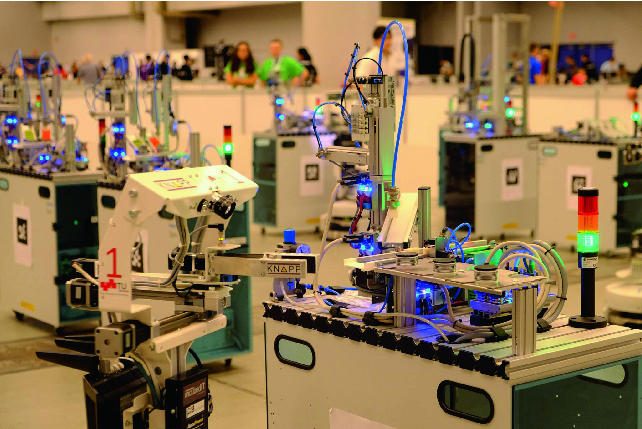
\includegraphics[scale=0.35]{NewFigures/RC_Logistics.png}
    %\caption{Ambiente Virtual}
    \label{fig:Robocup}
\end{figure}
\end{frame}

\begin{frame}{PLANTEAMIENTO DEL PROBLEMA}
%%%%         No Mod
El procedimiento propuesto se inspira en la competencia \textit{RoboCup Logistics League} que se realiza haciendo uso del robot Robotino de FESTO, en el cual un equipo de máximo 3 robots deben trabajar de manera colaborativa en la ejecución de diferentes tareas que componen la simulación de un proceso de producción industrial \cite{robocup__mathworks_robocup_2022}.
\phantom{sd}\\
\begin{figure}[htp]
    \centering
    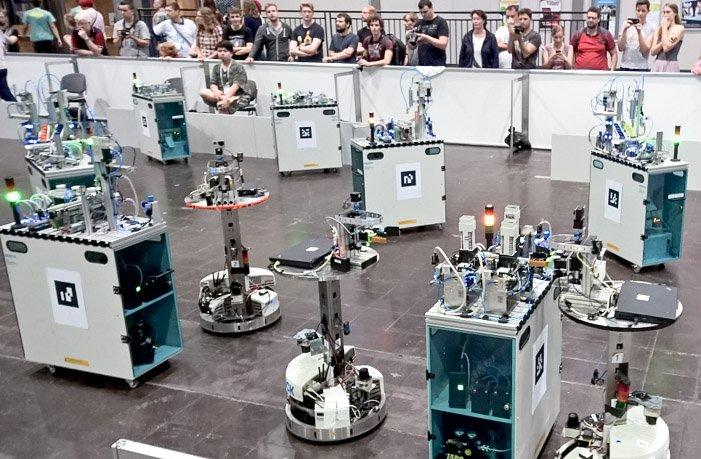
\includegraphics[scale=0.45]{NewFigures/RC_Logistics_2018.jpg}
    %\caption{Ambiente Virtual}
    \label{fig:Workspace}
\end{figure}
\end{frame}

\begin{frame}{PLANTEAMIENTO}

Procesamiento de los datos de los sensores del robot.\\
    %\begin{itemize}
     %   \item Procesamiento de imágenes.
      %  \item Visión computacional.
       % \item Sistemas expertos.
        %\item Planeación de acciones.
    %\end{itemize}
\begin{figure}[htp]
    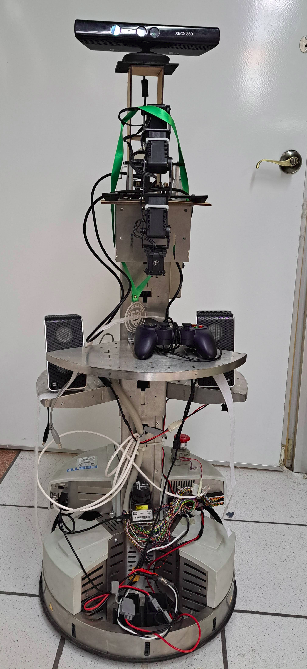
\includegraphics[scale=0.25]{NewerFigures/FestinoNew.png}
    %\caption{Ambiente Virtual}
    \label{fig:FestinoNew}
\end{figure}
\end{frame}


%------------------------------------------------------------------------------

%------------------------------------------------------------------------------


\section{Objetivos}
\begin{frame}{OBJETIVOS GENERALES}
\phantom{sd}\\
\begin{itemize}
    \item Procesar la imagen RGB.
    \item Procesar la nube de puntos  
    \item Planeación de la estrategia del ensamblado de objetos.
\end{itemize}
\begin{figure}[htp]
    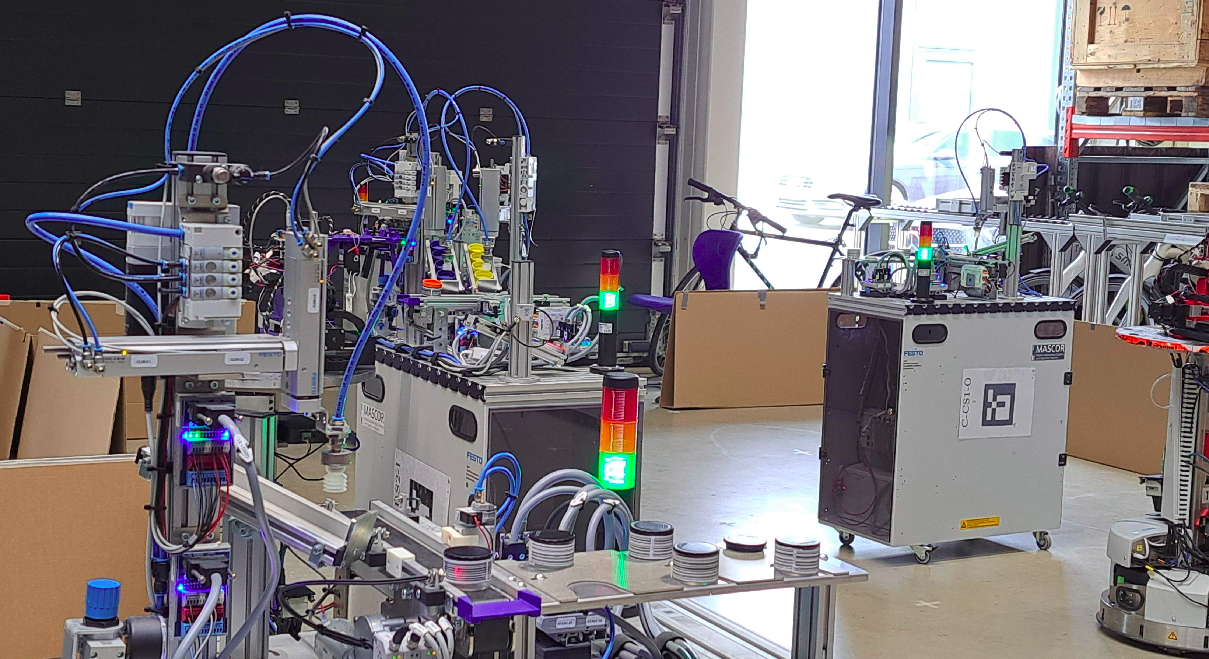
\includegraphics[scale=0.2]{NewerFigures/mps+arena.png}
    %\caption{Ambiente Virtual}
    \label{fig:LogisticsArena}
\end{figure}
\end{frame}
\begin{comment}

\end{comment}


%------------------------------------------------------------------------------

%------------------------------------------------------------------------------

\section{Metas}
\begin{frame}{METAS}
\phantom{sd}\\
\phantom{sd}\\
Se busca que los Robots de servicio para fábricas inteligentes: 
\begin{itemize}
    \item Realicen tareas útiles para humanos o robots en entornos industriales.
    \item Desempeñen tareas sencillas de forma colaborativa.
    \item Completen actividades distribuidas en etapas.
    \item Faciliten la automatización del proceso \cite{ifr_international_nodate}.
    \item Interactúen con objetos, equipamiento, humanos y otros robots. \cite{basco_industria_2018}.    
\end{itemize}
\end{frame}

%------------------------------------------------------------------------------

%------------------------------------------------------------------------------
\section{Metodología}
\begin{frame}{METODOLOGÍA}
    \begin{itemize}
    \item Usando técnicas de procesamiento de imágenes y utilizando de la nube de puntos se identificarán las entradas y salidas de las bandas transportadoras.
    \end{itemize}
 \begin{figure}[htp]
    \centering
    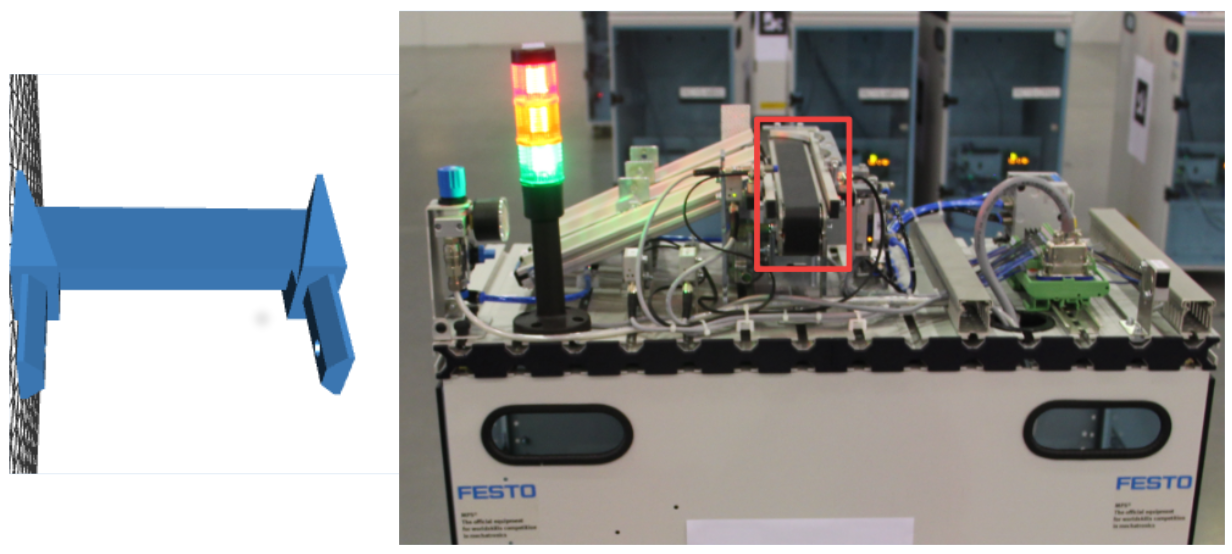
\includegraphics[scale=0.25]{NewFigures/Conveyor_Belt.png}
\end{figure}  
\end{frame}

\begin{frame}{METODOLOGÍA}
\begin{itemize}
    \item Segmentación por color de la imagen.
    \item Análisis de la nube de puntos: Posición relativa y orientación para recolección o depósito de los objetos. 
    \item Proceso de visión activa para optimizar la perspectiva de la cámara \cite{roveda_robot_2022}.
    \phantom{sd}\\
    \phantom{sd}\\
    \begin{figure}[htp]
    \centering
    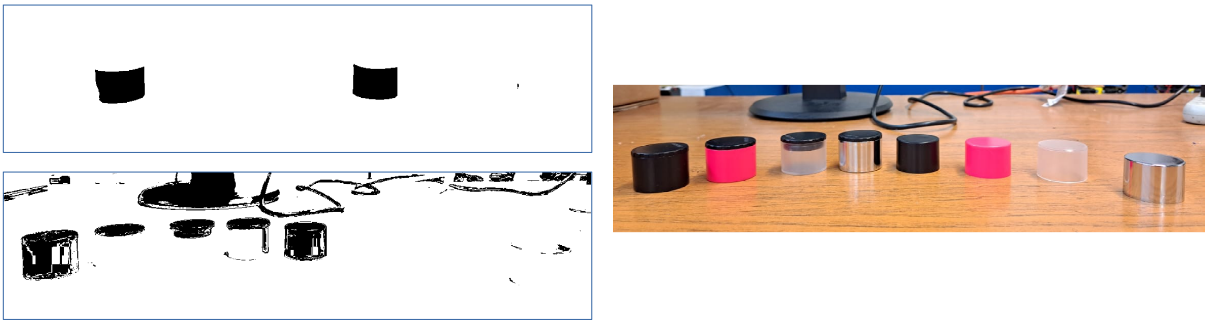
\includegraphics[scale=0.25]{NewFigures/Filtered_R_B.png}
\end{figure}
    
\end{itemize}
\end{frame}

\begin{frame}{METODOLOGÍA}
\begin{itemize}
    \item El gripper previamente planteado fue reemplazado con un  brazo robótico PhantomX Pincher, por lo que fue realizada la reintegración de la paquetería moveit para su control. De esta forma, al brazo le es entregada una coordenada referente a un sistema de coordenadas y adopta dicha posición. Los cálculos referentes al movimiento de los actuadores se realizan dentro de la paquetería.\\
    \phantom{sd}

\end{itemize}
\begin{figure}[htp]
    \centering
    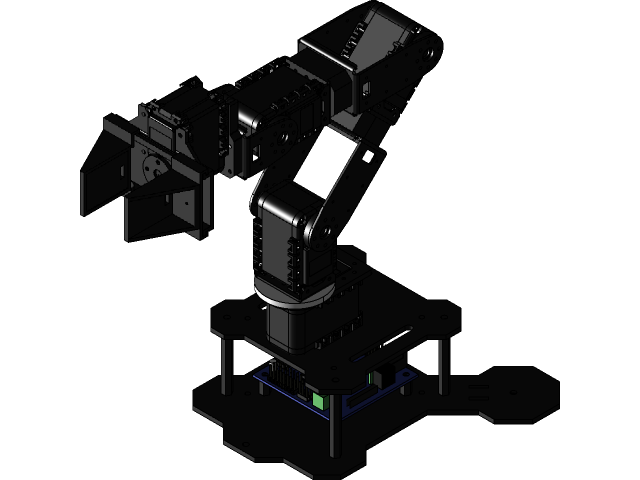
\includegraphics[scale=0.2]{NewerFigures/phantom.png} 
\end{figure}
\end{frame}

\begin{frame}{METODOLOGÍA}
\begin{figure}[htp]
    \centering
    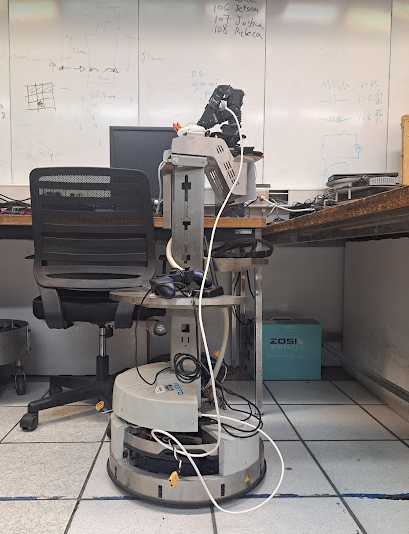
\includegraphics[scale=0.35]{NewerFigures/phantom+table.png} 
\end{figure}
\end{frame}

\begin{frame}{METODOLOGÍA}
Se utilizará un algoritmo basado en reglas y la información que haya sido introducida al robot a forma de conocimiento (sistema experto) \cite{giarratano_expert_2006}, para realizar la planeación de la tarea de manipulación. \\
Ejemplos de indicaciones a seguir recibidas por Protocol Buffer:
\begin{itemize}
    \item C-SS contains: (0 3) stores BASE\_RED CAP\_GREY
    \item Ring color RING\_YELLOW requires 2 additional bases
\end{itemize}
\begin{figure}[htp]
    \centering
    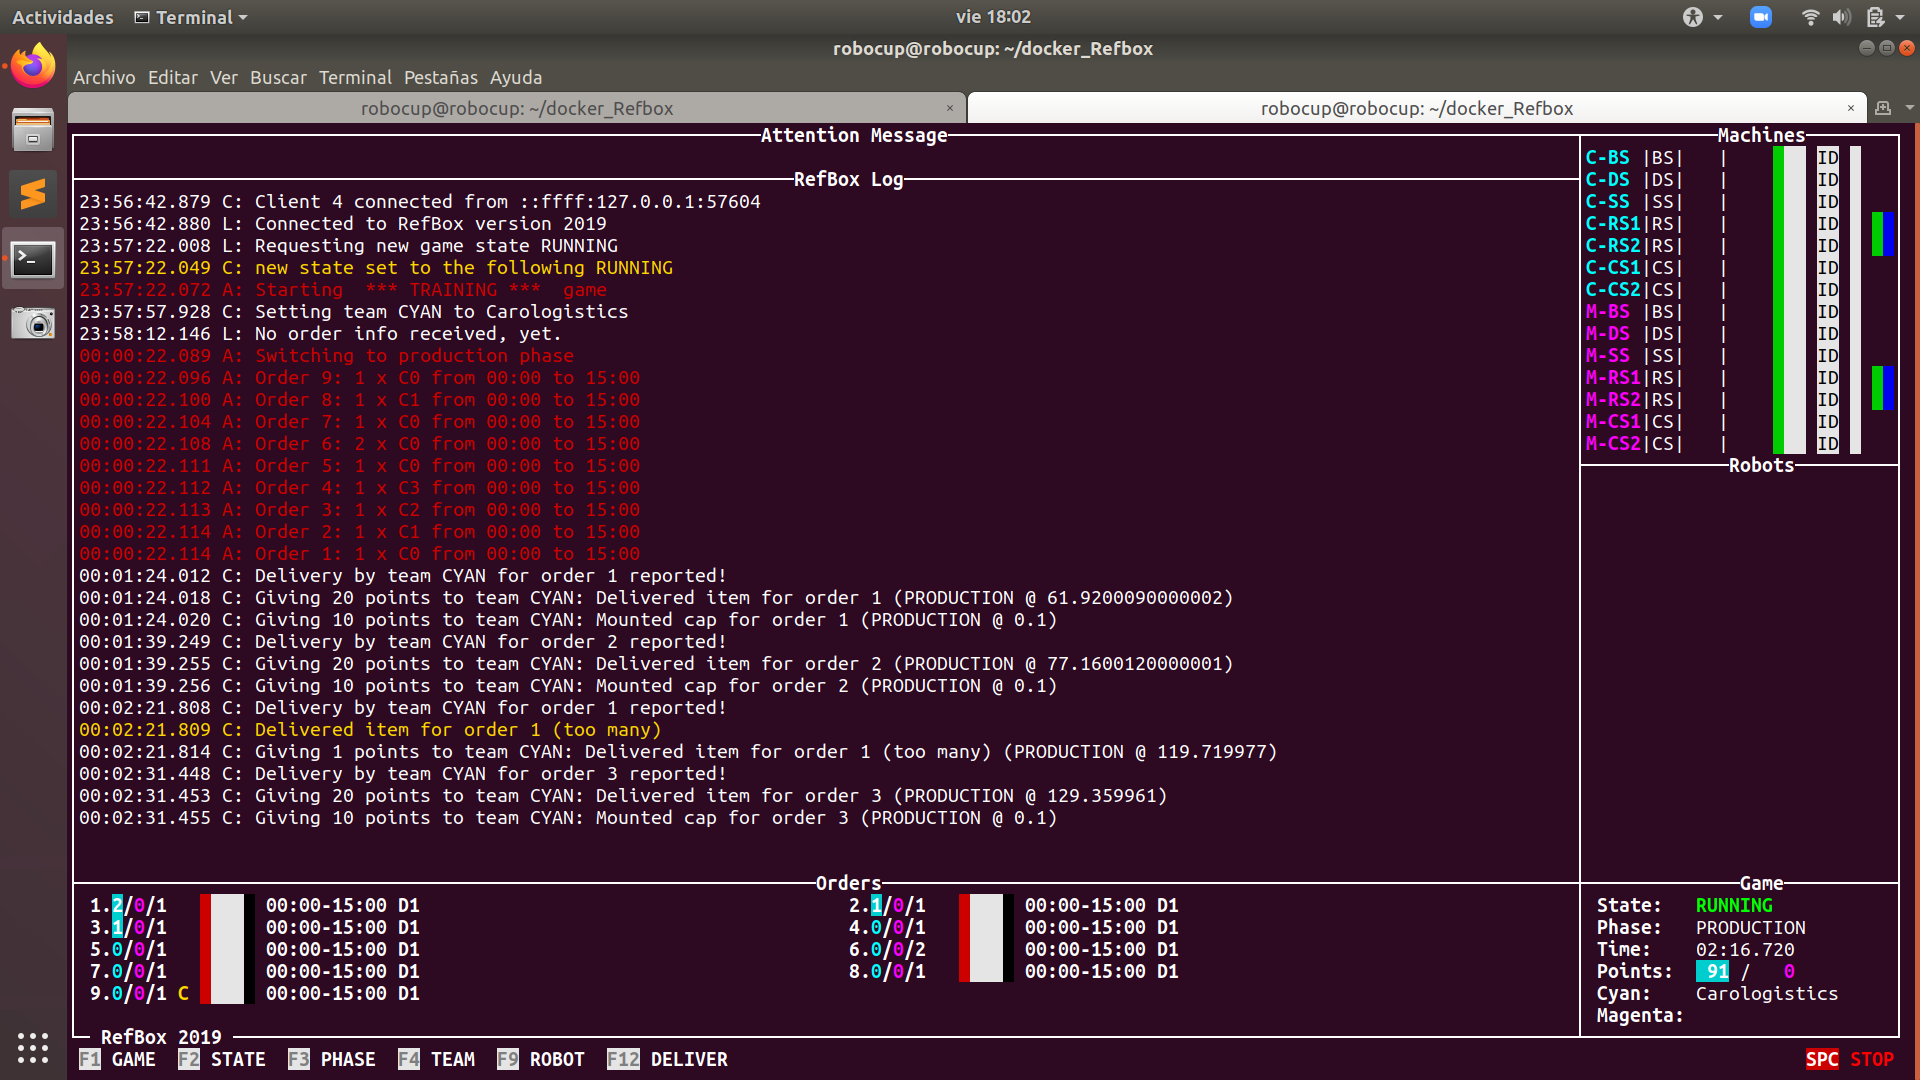
\includegraphics[scale=0.1]{NewFigures/Refbox_1.png}
\end{figure}
\end{frame}
\begin{frame}{HARDWARE}
\begin{itemize}
    \item Reemplazo de la pinza con manipulador
    \item Recableado de la alimentación / reemplazo de baterías
    \item Puesta en marcha del sistema de comunicación con el RefBox
    \item Acondicionamientos de altura y distribución del robot
    \item Bases para elementos periféricos
\end{itemize}
\begin{figure}[htp]
    \centering
    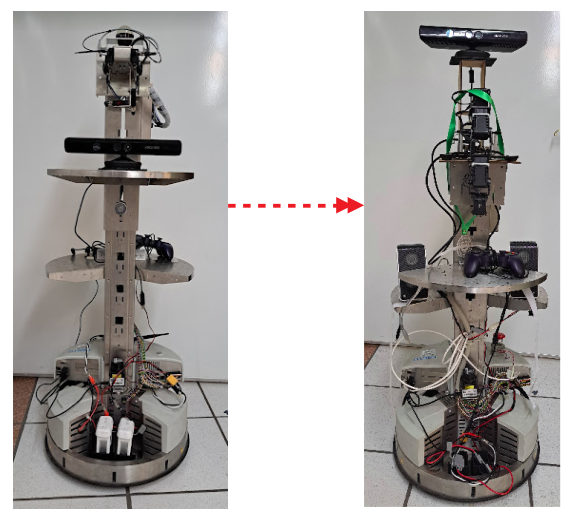
\includegraphics[scale=0.25]{NewerFigures/GlowUp.png}
\end{figure}
\end{frame}
\begin{frame}{HERRAMIENTAS}
\phantom{sd}\\
\phantom{sd}\\
\begin{itemize}
    \item Procesamiento de imagen - OpenCV y NumPy.
    \item Clasificación de objetos - Histograma de color.
    \item Planeación de acciones, Sistema experto - CLIPS.
    \item Cinemática inversa, Nube de Puntos - MoveIt y Octomap \cite{hornung_octomap_2013}
    \item Integración - Robot Opearating System (ROS)
    \item Protocol Buffer
    \item Robotino View
\end{itemize}
\end{frame}

%------------------------------------------------------------------------------

%------------------------------------------------------------------------------
%trim={<izquierda> <abajo> <derecha> <arriba>}

%------------------------------------------------------------------------------

\begin{frame}{REFERENCIAS}
\printbibliography 
\end{frame}
\end{document}
